% -*- mode: latex; mode: visual-line; fill-column: 9999; coding: utf-8 -*-

\section{Algorithms and Software Packages}
\label{sec:packages}

For our investigation of parallel trajectory analysis we focus on using MPI as the standard approach to parallelization in HPC.
We employ the Python language, which is widely used in the scientific community because it facilitates rapid development of small scripts and code prototypes as well as development of large applications and highly portable and reusable modules and libraries.
We use the \package{MDAnalysis} library to calculate a ``RMSD timeseries'' (explained in section \ref{sec:mda}) as a representative use case.
Further details on the software packages are provided in sections \ref{sec:methods-mpi4py}--\ref{sec:methods-hdf5}.


\subsection{RMSD Calculation with MDAnalysis}
\label{sec:mda}

Simulation data exist in trajectories in the form of time series of atom positions and sometimes velocities.
Trajectories come in a plethora of different and idiosyncratic file formats. 
\package{MDAnalysis} \cite{Gowers:2016aa, Michaud-Agrawal:2011fu} is a widely used open source library to analyze trajectory files with an object oriented interface. 
The library is written in Python, with time critical code in C/C++/Cython. 
\package{MDAnalysis} supports most file formats of simulation packages including CHARMM \cite{Brooks:2009pt}, Gromacs \cite{Abraham:2015aa}, Amber \cite{Case:2005uq}, and NAMD \cite{Phillips:2005ek} and the Protein Data Bank \cite{Burley:2018aa} format.
At its core, it reads trajectory data in different formats and makes them available through a uniform API; specifically, coordinates are represented as standard NumPy arrays \cite{Van-Der-Walt:2011aa}.


\begin{figure}[!htb]
  \centering
  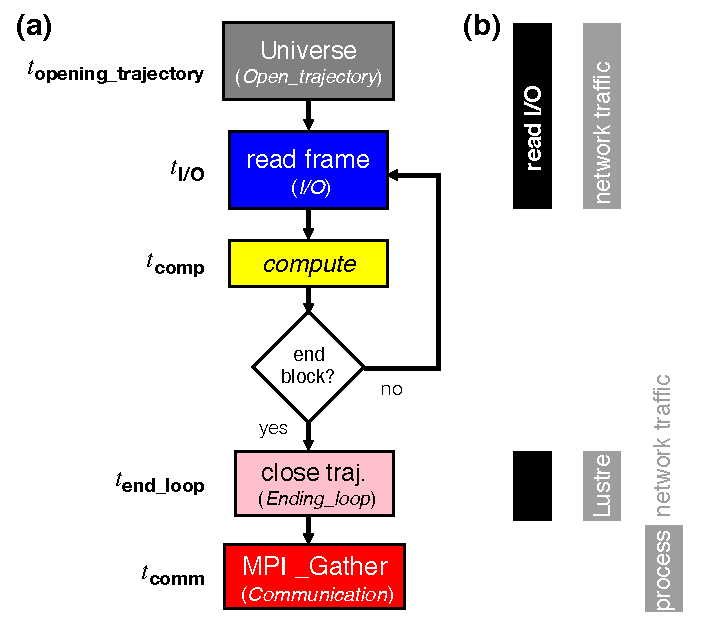
\includegraphics[width=7cm]{figures/flowchart.pdf}
  \caption{Flow chart of the MPI-parallelized RMSD algorithm, Algorithm~\ref{alg:RMSD}.
    \textbf{(a)} Each MPI process performs the same steps but reads trajectory frames from different blocks of the trajectory.
    The color scheme and labels in italics correspond to the colors and labels for measured timing quantitities in the following graphs (e.g., Figs.~\protect\ref{fig:ScalingComputeIO} and \protect\ref{fig:MPIranks}).
    The names of the corresponding timing quantitities from Table \protect\ref{tab:notation} are listed next to each step.
    \textbf{(b)} Steps that access the shared Lustre file system with read I/O are included in the black bars; steps that communicate via the shared InfiniBand network are included in the gray bars.
    The Lustre file system is accessed through the network and hence all I/O steps also use the network.
  }
  \label{fig:flowchart}
\end{figure}

As a test case that is representative of a common task in the analysis of biomolecular simulation trajectories we calculated the timeseries of the minimal structural root mean square distance  (\textbf{RMSD}) after rigid body superposition \cite{Lea96, Mura:2014kx}.
The RMSD is used to show the rigidity of protein domains and more generally characterizes structural changes.
It is calculated as a function of time $t$ as
\begin{equation}
  \label{eq:rmsd}
  \text{RMSD}(t) = \min_{\mathsf{R}, \mathbf{t}} %
  \sqrt{\frac{1}{N} \sum_{i=1}^{N} \left[ %
      (\mathsf{R}\cdot\mathbf{x}_{i}(t) + \mathbf{t}) - \mathbf{x}_{i}^{\text{ref}} \right]^{2}}
\end{equation}
where $\mathbf{x}_{i}(t)$ is the position of atom $i$ at time $t$, $\mathbf{x}_{i}^{\text{ref}}$ is its position in a reference structure and the distance between these two is minimized by finding the optimum $3\times3$ rotation matrix $\mathsf{R}$ and translation vector $\mathbf{t}$. 
The optimum rigid body superposition was calculated with the QCPROT algorithm~\cite{Liu:2010kx,Theobald:2005vn} (implemented in Cython and available through the \texttt{MDAnalysis.analysis.rms} module \cite{Gowers:2016aa}).

The RMSD trajectory analysis was parallelized as outlined in the flow chart in Figure~\ref{fig:flowchart}, with further details available in Algorithm~\ref{alg:RMSD}.
Each MPI process loads the core MDAnalysis structure (called the \texttt{Universe}), which includes loading a shared ``topology'' file with the simulation system information and opening the shared trajectory file.
Each process operates on a different block of frames and iterates through them by reading the coordinates of a single frame into memory and performing the RMSD computation with them.
Once all frames in the block are processed, the trajectory file is closed and results are communicated to MPI rank 0 using \texttt{MPI\_Gather()}.

The RMSD was determined for a subset of protein atoms, the $N=214$  C$_{\alpha}$ atoms of our test system (see section \ref{sec:data} for details).
The time complexity for the RMSD Algorithm~\ref{alg:RMSD} is $\mathcal{O}(T \times N^{2})$~\cite{Liu:2010kx} where $T$ is the number of frames in the trajectory and $N$ the number of particles included in the RMSD calculation.

\begin{algorithm}[ht!]
	\scriptsize
	\caption{MPI-parallel Multi-frame RMSD Algorithm}
	\label{alg:RMSD}
	\hspace*{\algorithmicindent} \textbf{Input:} \emph{size}: Total number of frames \\
	\hspace*{\algorithmicindent} \emph{ref}: mobile group in the initial frame which will be considered as reference \\
	\hspace*{\algorithmicindent} \emph{start \& stop}: Starting and stopping frame index\\
	\hspace*{\algorithmicindent} \emph{topology \& trajectory}: files to read the data structure from \\
	\hspace*{\algorithmicindent} \textbf{Output:} Calculated RMSD arrays
	\begin{algorithmic}[1]
		\Procedure{$Block\_RMSD$}{topology, trajectory, $ref$, start, stop}                       
		\State u $\leftarrow$ Universe(topology, trajectory)\Comment{u hold all the information of the physical system}
		\State $g$ $\leftarrow$ u.frames[start:stop]
		\For{$\forall iframe$ in $g$}
		\State $results[iframe] \leftarrow RMSD(g, ref)$
		\EndFor
		\State \Return results
		\EndProcedure
		\\        
		\State MPI Init
		\State rank $\leftarrow$ rank ID
		\State index $\leftarrow$ indices of mobile atom group
		\State xref0 $\leftarrow$ Reference atom group\textsc{\char13}s position
		\State out $\leftarrow$ Block\_RMSD(topology, trajectory, xref0, start=start, stop=stop)
		\\
		\State Gather(out, RMSD\_data, rank\_ID=0)
		\State MPI Finalize
	\end{algorithmic}
\end{algorithm}


\subsection{MPI for Python (\package{mpi4py})}
\label{sec:methods-mpi4py}

MPI for Python (\package{mpi4py}) is a Python wrapper for the Message Passing Interface (MPI) standard and allows any Python program to employ multiple processors \cite{Dalcin:2011aa, Dalcin:2005aa}.
Performance degradation due to using \package{mpi4py} is not prohibitive \cite{Dalcin:2011aa, Dalcin:2005aa} and the overhead is far smaller than the overhead associated with the use of interpreted versus compiled languages \cite{GAiN}.
Overheads in \package{mpi4py} are small compared to C code if efficient raw memory buffers are used for communication \cite{Dalcin:2011aa}, as used in the present study.

\subsection{Global Arrays Toolkit}
\label{sec:methods-ga}

The \package{Global Arrays} (GA) toolkit provides users with a language interface that allows them to distribute data while maintaining the type of global index space and programming syntax similar to what is available when programming on a single processor \cite{GA}.
\emph{Global Arrays} is implemented with Fortran-77 and C bindings and provides C++ and Python interfaces.
It allows manipulating physically distributed dense multi-dimensional arrays without explicitly defining communication and synchronization between processes.
The underlying communication is determined by a runtime environment, which defaults to the \emph{Communication runtime for Extreme Scale} (ComEx) \cite{Daily:2014aa}.
ComEx uses shared memory for intra-node communication and inter-node communication employs ComEx with MPI.
\emph{Global Arrays in NumPy} (GAiN) extends GA to Python through Numpy \cite{GAiN}. 
The \package{Global Arrays} toolkit provides functions to create global arrays (\texttt{ga\_create()}) and to copy data to (\texttt{ga\_put()}) and from (\texttt{ga\_get()}) such a global array,  as well as additional functions for copying between arrays and freeing them \cite{GAiN}.
When a global array is created (\texttt{ga\_create()}) each process will create an array of the same shape and size, physically located in the local memory space of that process \cite{GA}. 
The GA library maintains a list of all these memory locations, which can be queried with the \texttt{ga\_access()} function.
Using a pointer returned by \texttt{ga\_access()}, one can directly modify the data that is local to each process.
When a process tries to access a block of data the request is first decomposed into individual blocks representing the contribution to the total request from the data held locally on each process (\textit{B. J. Palmer and J. Daily, personal communication}).
The requesting process then makes individual requests to each of the remote processes. 

GA allows independent, asynchronous, and efficient access to logical blocks of physically distributed arrays, with no need for explicit cooperation by other processes; in particular, it allows data locality to be explicitly specified and used \cite{GA-NUMA}.
We investigated if communication cost could be reduced by using \package{Global Arrays}.
Algorithm \ref{alg:GA} describes the RMSD algorithm with \package{Global Arrays} instead of MPI.


\begin{algorithm}[ht!]
	\scriptsize
	\caption{MPI-parallel Multi-frame RMSD using Global Arrays}
	\label{alg:GA}
	\hspace*{\algorithmicindent} \textbf{Input:}\emph{size}: Total number of frames assigned to each rank $N_{b}$\\
	\hspace*{\algorithmicindent} \emph{g\_a}: Initialized Global Arrays \\
	\hspace*{\algorithmicindent} \emph{xref0}: mobile group in the initial frame which will be considered as reference \\
	\hspace*{\algorithmicindent} \emph{start \& stop}: that tell which block of trajectory (frames) is assigned to each rank \\
	\hspace*{\algorithmicindent} \emph{topology \& trajectory}: files to read the data structure from \\
	\hspace*{\algorithmicindent}\textbf{Include:} \texttt{Block\_RMSD()} from Algorithm \ref{alg:RMSD}
	\begin{algorithmic}[1]
		
		\State bsize $\leftarrow$ ceil(trajectory.number\_frames / size)
		\State g\_a $\leftarrow$ ga.create(ga.C\_DBL, [bsize*size,2], "RMSD")
		\State buf $\leftarrow$ np.zeros([bsize*size,2], dtype=float)
		\State out $\leftarrow$ Block\_RMSD(topology, trajectory, xref0, start=start, stop=stop)
		\State ga.put(g\_a, out, (start,0), (stop,2))
		\If{rank == 0}
		\State buf $\leftarrow$ ga.get(g\_a, lo=None, hi=None)
		\EndIf
	\end{algorithmic}
\end{algorithm}

\subsection{MPI and Parallel HDF5}
\label{sec:methods-hdf5}

HDF5 is a structured self-describing hierarchical data format which is the standard mechanism for storing large quantities of numerical data in Python (\url{http://www.hdfgroup.org/HDF5}, \cite{pythonhdf5}).
Parallel HDF5 (\package{PHDF5}) typically sits on top of a MPI-IO layer and can use MPI-IO optimizations. 
In \package{PHDF5}, all file access is coordinated by the MPI library; otherwise, multiple processes would compete over accessing the same file on disk. 
MPI-based applications launch multiple parallel instances of the Python interpreter that communicate with each other via the MPI library. 
Implementation is straightforward as long as the user supplies a MPI communicator and takes into account some constraints required for data consistency \cite{pythonhdf5}.
\package{HDF5} itself handles nearly all the details involved with coordinating file access when the shared file is opened through the \emph{mpio} driver.

MPI has two flavors of operation: collective (all processes have to participate in the same order) and independent (processes can perform the operation in any order or not at all) \cite{pythonhdf5}.
With \package{PHDF5}, modifications to file metadata must be performed collectively and although all processes perform the same task, they do not need to be synchronized \cite{pythonhdf5}. 
Other tasks and any type of data operations can be performed independently by processes.
In the present study, we use independent operations.
